\documentclass[a0paper,portrait]{baposter-metu}

\usepackage{lipsum}          % This is just for some blindtext

\usepackage{relsize}	       % For \smaller
\usepackage{url}			       % For \url
\usepackage{epstopdf}	       % Included EPS files automatically converted to PDF to include with pdflatex
\usepackage{multicol}        % Multi Columns

\usepackage{amsmath,amssymb} % math

%%%%%%%%%%%%%%%%%%%%%%%%%%%%%%%%%%%%%%%%%%%%%%%%%%%%%%%%%%%%%%%%%%%%%%%%%%%%%%%%
%%% Utility functions %%%%%%%%%%%%%%%%%%%%%%%%%%%%%%%%%%%%%%%%%%%%%%%%%%%%%%%%%%
%%%%%%%%%%%%%%%%%%%%%%%%%%%%%%%%%%%%%%%%%%%%%%%%%%%%%%%%%%%%%%%%%%%%%%%%%%%%%%%%

%%% Save space in lists. Use this after the opening of the list %%%%%%%%%%%%%%%%
\renewcommand{\vec}[1]{\bm{#1}}
\newcommand{\vnabla}{\vec{\nabla}}

\renewcommand{\d}[1]{\text{d} #1}
\newcommand{\dxx}{\,\text{d}\vec{x}}
\newcommand{\dx}{\,\text{d}x}

\newcommand{\diff}[2]{\frac{\text{d}#1}{\text{d}#2}}
\newcommand{\idiff}[2]{\text{d}#1 / \text{d}#2}
\newcommand{\pdiff}[2]{\frac{\partial #1}{\partial #2}}
\newcommand{\pdifff}[2]{\frac{\partial^2 #1}{\partial #2^2}}
\newcommand{\ipdiff}[2]{\partial #1 / \partial #2}
\newcommand{\vdiff}[2]{\frac{\delta #1}{\delta #2}}
\newcommand{\ivdiff}[2]{\delta #1 / \delta #2}

%%%%%%%%%%%%%%%%%%%%%%%%%%%%%%%%%%%%%%%%%%%%%%%%%%%%%%%%%%%%%%%%%%%%%%%%%%%%%%%
%%% Document Start %%%%%%%%%%%%%%%%%%%%%%%%%%%%%%%%%%%%%%%%%%%%%%%%%%%%%%%%%%%%
%%%%%%%%%%%%%%%%%%%%%%%%%%%%%%%%%%%%%%%%%%%%%%%%%%%%%%%%%%%%%%%%%%%%%%%%%%%%%%%

\begin{document}
\typeout{Poster rendering started}

%%% General Poster Settings %%%%%%%%%%%%%%%%%%%%%%%%%%%%%%%%%%%%%%%%%%%%%%%%%%%
%%%%%% Eye Catcher, Title, Authors and University Images %%%%%%%%%%%%%%%%%%%%%%
\begin{poster}{
  columns=2,
	grid=false,
	borderColor=metudarkblue,
	headerColorOne=metudarkblue,
	headerColorTwo=metudarkblue,
	headerFontColor=metulight,
  headerheight=14em,
	boxColorOne=white,
  boxpadding=1em,
	headershape=rounded,
	headerfont=\Large\textsf,
	textborder=rounded,
	background=shadetb,
  bgColorOne=metulight!10,
  bgColorTwo=metudarkblue!30,
	headerborder=open,
  boxshade=plain,
  eyecatcher=false
}
%%% Eye Cacther %%%%%%%%%%%%%%%%%%%%%%%%%%%%%%%%%%%%%%%%%%%%%%%%%%%%%%%%%%%%%%%
{
}
%%% Title %%%%%%%%%%%%%%%%%%%%%%%%%%%%%%%%%%%%%%%%%%%%%%%%%%%%%%%%%%%%%%%%%%%%%
{\smaller \textcolor{metured}{Balancing error and scaling in  Quantum Discord\\ in a quantum computer with machine learning}}
%%% Authors %%%%%%%%%%%%%%%%%%%%%%%%%%%%%%%%%%%%%%%%%%%%%%%%%%%%%%%%%%%%%%%%%%%
{
  \vspace{1em} \textcolor{metudark}{
   	K. Aytemiz, C. Kehribar, Ö. Nazlı, K, Yurtseven, Z. Çırnaz, T, Yücel,  O.B. Malcioglu*\\
	{\smaller *mbaris@metu.edu.tr}
}}
%%% Logo %%%%%%%%%%%%%%%%%%%%%%%%%%%%%%%%%%%%%%%%%%%%%%%%%%%%%%%%%%%%%%%%%%%%%%
{
\begin{minipage}{20.0em}
    
\includegraphics[height=12em]{METU-short-transparent}
  \end{minipage}
}

%%% Second Quantum Revolution %%%%%%%%%%%%%%%%%%%%%%%%%%%%%%%%%%%%%%%%%%%%%%%%%%%%%%%%%%%%%%%%%%
\headerbox{Second Quantum Revolution}{name=sqr,column=0,row=0}{
  \textbf{We’re in the midst of a new revolution in quantum physics.} The first revolution enabled inventions such as the laser and transistor, the basic building block of computers, when scientists knew the rules of quantum mechanics and built devices that followed those rules. The second quantum revolution is all about controlling individual quantum systems, such as charged molecules, to a greater extent than before, enabling even more powerful applications of quantum information theory. \\

    \centering
    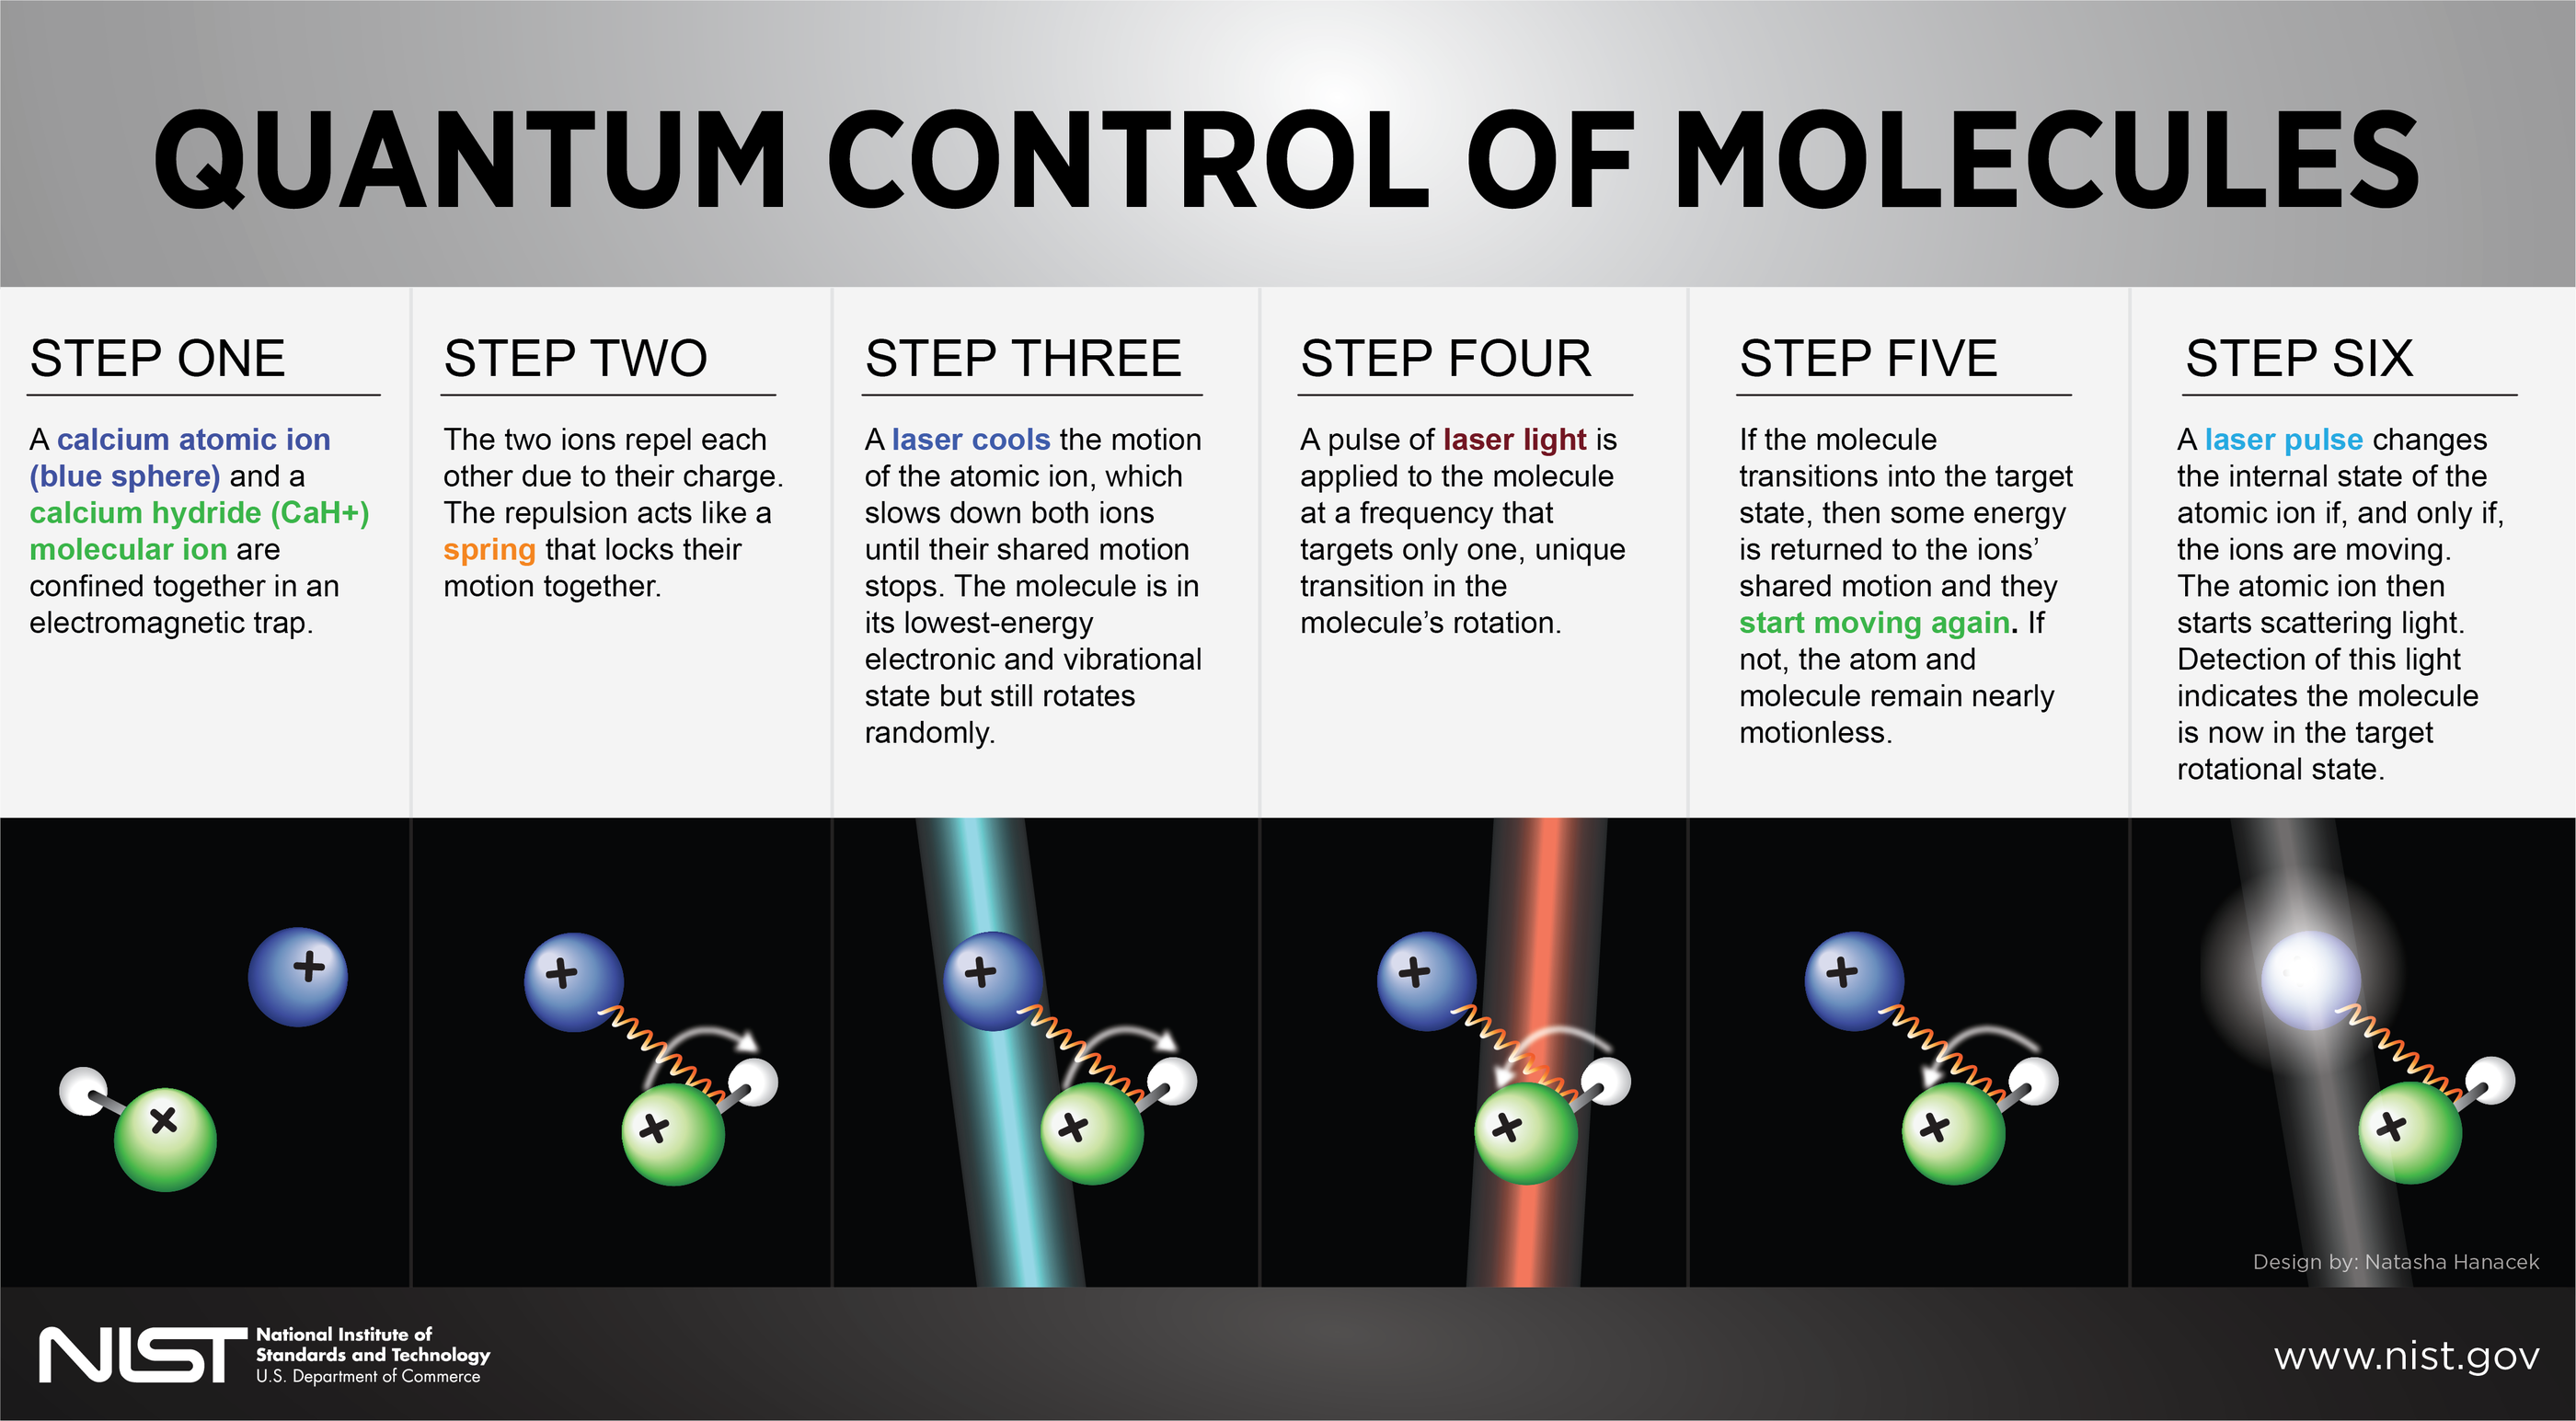
\includegraphics[width=\linewidth]{17pml002_molec_ion_infographic_hr.png}
}
%%% Quantum Discord %%%%%%%%%%%%%%%%%%%%%%%%%%%%%%%%%%%%%%%%%%%%%%%%%%%%%%%%%%%%%%%%%%
\headerbox{Quantum Discord}{name=qd,column=1,row=0}{
\textbf {A handy tool from Quantum information theory:}\\

 \begin{columns}
    \column{0.4\textwidth}
    \center{
    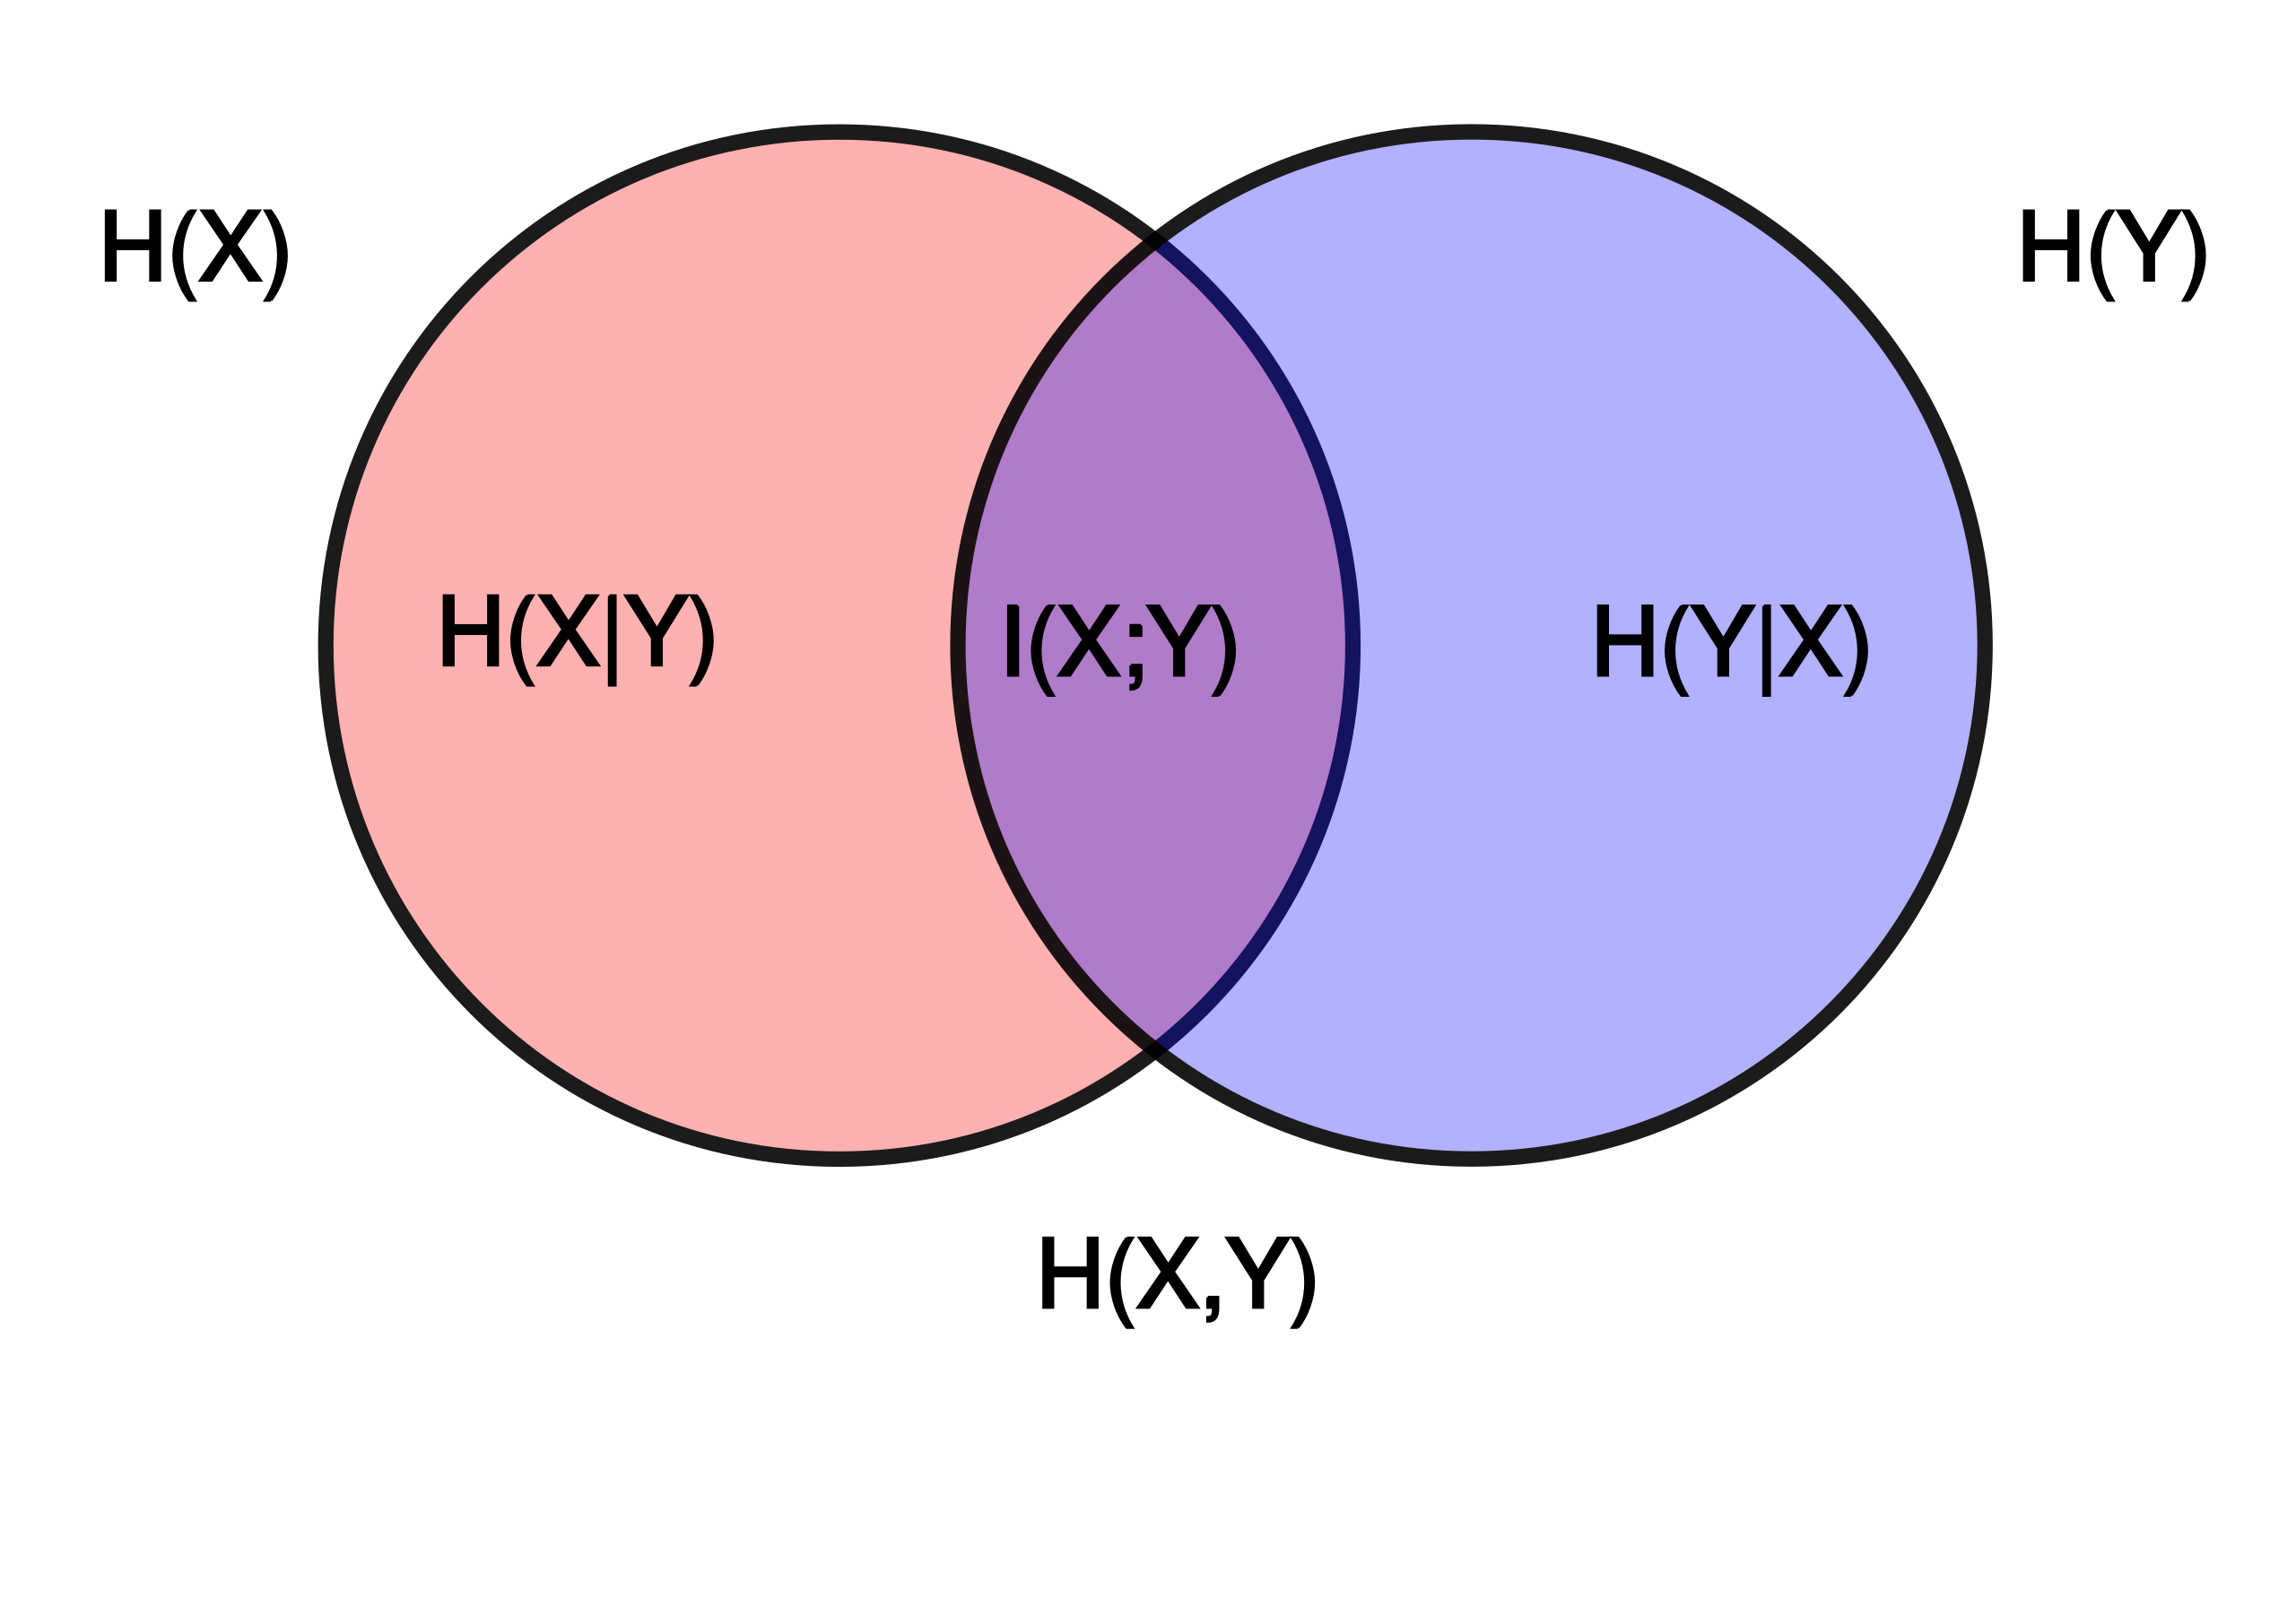
\includegraphics[height=10em]{Entropy-mutual-information-relative-entropy-relation-diagram.svg.png} }

    \column{0.6\textwidth}
Quantum discord [Phys. Rev. Lett. 88, 017901 (2001)], is a measure of the discrepancy between classical and quantum mutual information. It characterizes and quantifies quantumness of correlations in bipartite states from a measurement perspective. The phenomenon of nonzero quantum discord is a manifestation of quantum correlations due to noncommutativity rather than due to entanglement, and 
\end{columns}
 has interesting and significant applications in molecular systems, such as quantifying aromaticity, dynamic correlations effects such as FRET etc. However, calculation of Quantum Discord is NP-Hard and needs various approximation in traditional computing.
}
%%% Quantum Computers %%%%%%%%%%%%%%%%%%%%%%%%%%%%%%%%%%%%%%%%%%%%%%%%%%%%%%%%%%%%%%%%%%%%%
\headerbox{Quantum Computers}{name=QC,column=0,below=sqr}{
  \begin{columns}
    \column{0.4\textwidth}
    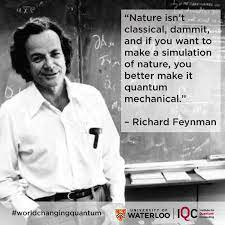
\includegraphics[width=1\linewidth]{index.jpg}
    \column{0.6\textwidth}
A quantum computer is a computer that takes advantage of quantum mechanical phenomena. The current state of quantum computing is referred to as the noisy intermediate-scale quantum (NISQ) era. These processors, are sensitive to their environment (noisy) and prone to quantum decoherence, are not yet capable of continuous quantum error correction. The noise issue gets exponentially worse in entangled systems (i.e. when there is quantum advantage over traditional computers)    
  \end{columns}%
    
}
%%% Classical Shadows %%%%%%%%%%%%%%%%%%%%%%%%%%%%%%%%%%%%%%%%%%%%%%%%%%%%%%%%%%%%%%%%%%%%%
\headerbox{Classical Shadows}{name=CS,column=0,below=QC}{
  \begin{columns}
    \column{0.6\textwidth}
    In principle, any unknown quantum state can be fully characterized by quantum state tomography. However, this procedure requires accurate expectation values for a set of observables whose size grows exponentially with the number of qubits. A potential workaround for these scaling concerns is provided by the classical shadow approximation introduced in a recent paper by Huang et al.  The classical shadow can be used to estimate properties two-point correlators hence Discord.
    \column{0.4\textwidth}
   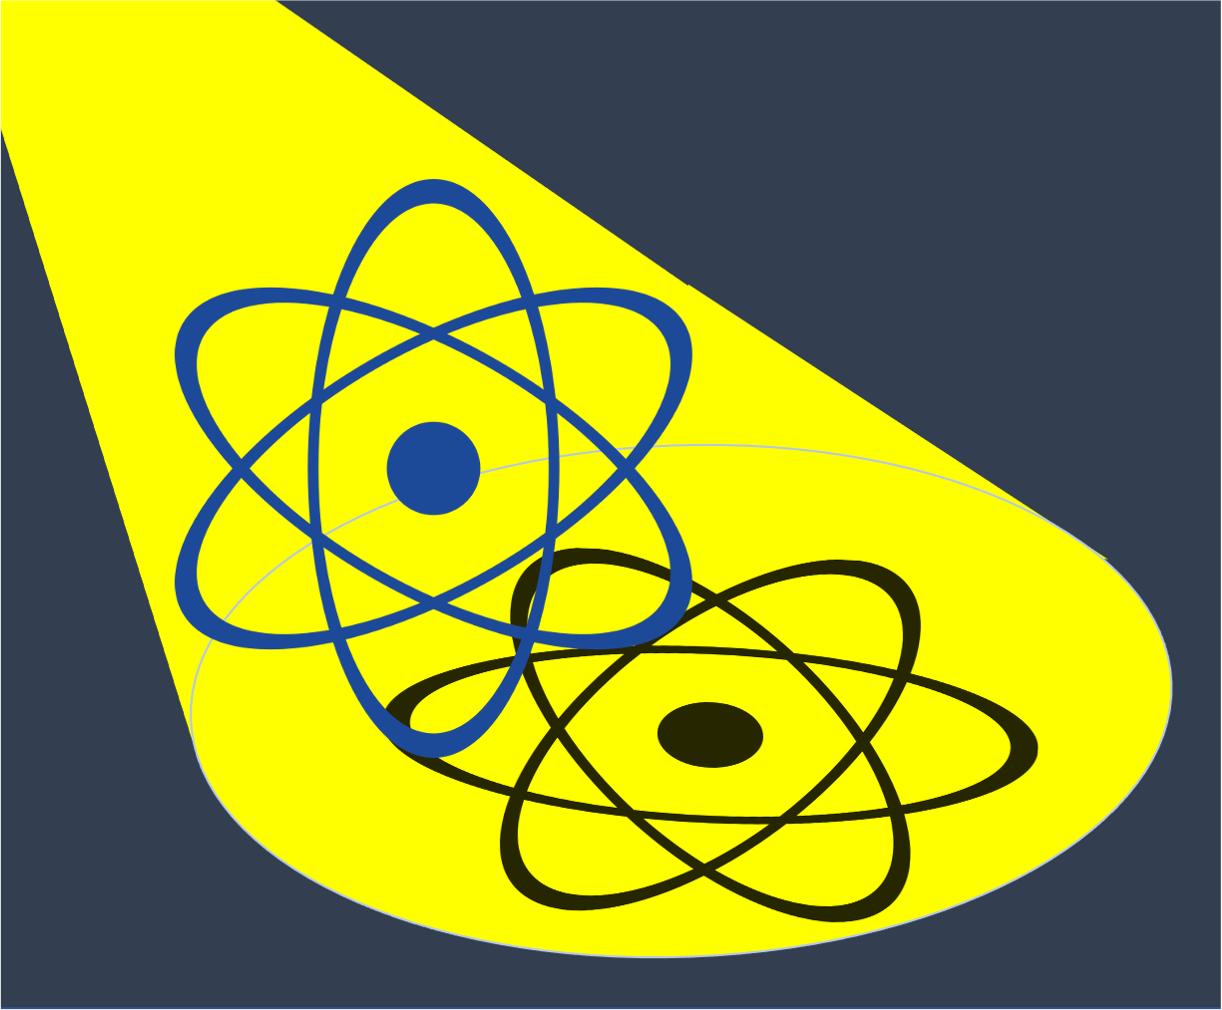
\includegraphics[width=1\linewidth]{atom_shadow.png}
  \end{columns}%
    
}
%%% Follow US %%%%%%%%%%%%%%%%%%%%%%%%%%%%%%%%%%%%%%%%%%%%%%%%%%%%%%%%%%%%%%%%%%%%%
\headerbox{Follow us in GitHub}{name=follow,column=0,below=CS,above=bottom}{
 \centering
    
\includegraphics[height=10em]{TDLDEFA-QUN-github.png}

    
}
%%% Machine learning %%%%%%%%%%%%%%%%%%%%%%%%%%%%%%%%%%%%%%%%%%%%%%%%%%%%%%%%%%%%%%%%%%%%%
\headerbox{Error mitigation with ML}{name=ML,column=1,below=qd}{
Machine learning models such as linear regression, random forests, multi-layer perceptrons, and graph neural networks are used to mitigate error on diverse classes of quantum circuits. Haoran Liao et al.  shows  how to scale ML-QEM to classically intractable quantum circuits by mimicking the results of traditional mitigation results, while significantly reducing overhead, suggesting a QPU+HPC advantage for calculating the quantum discord.  
\center{
    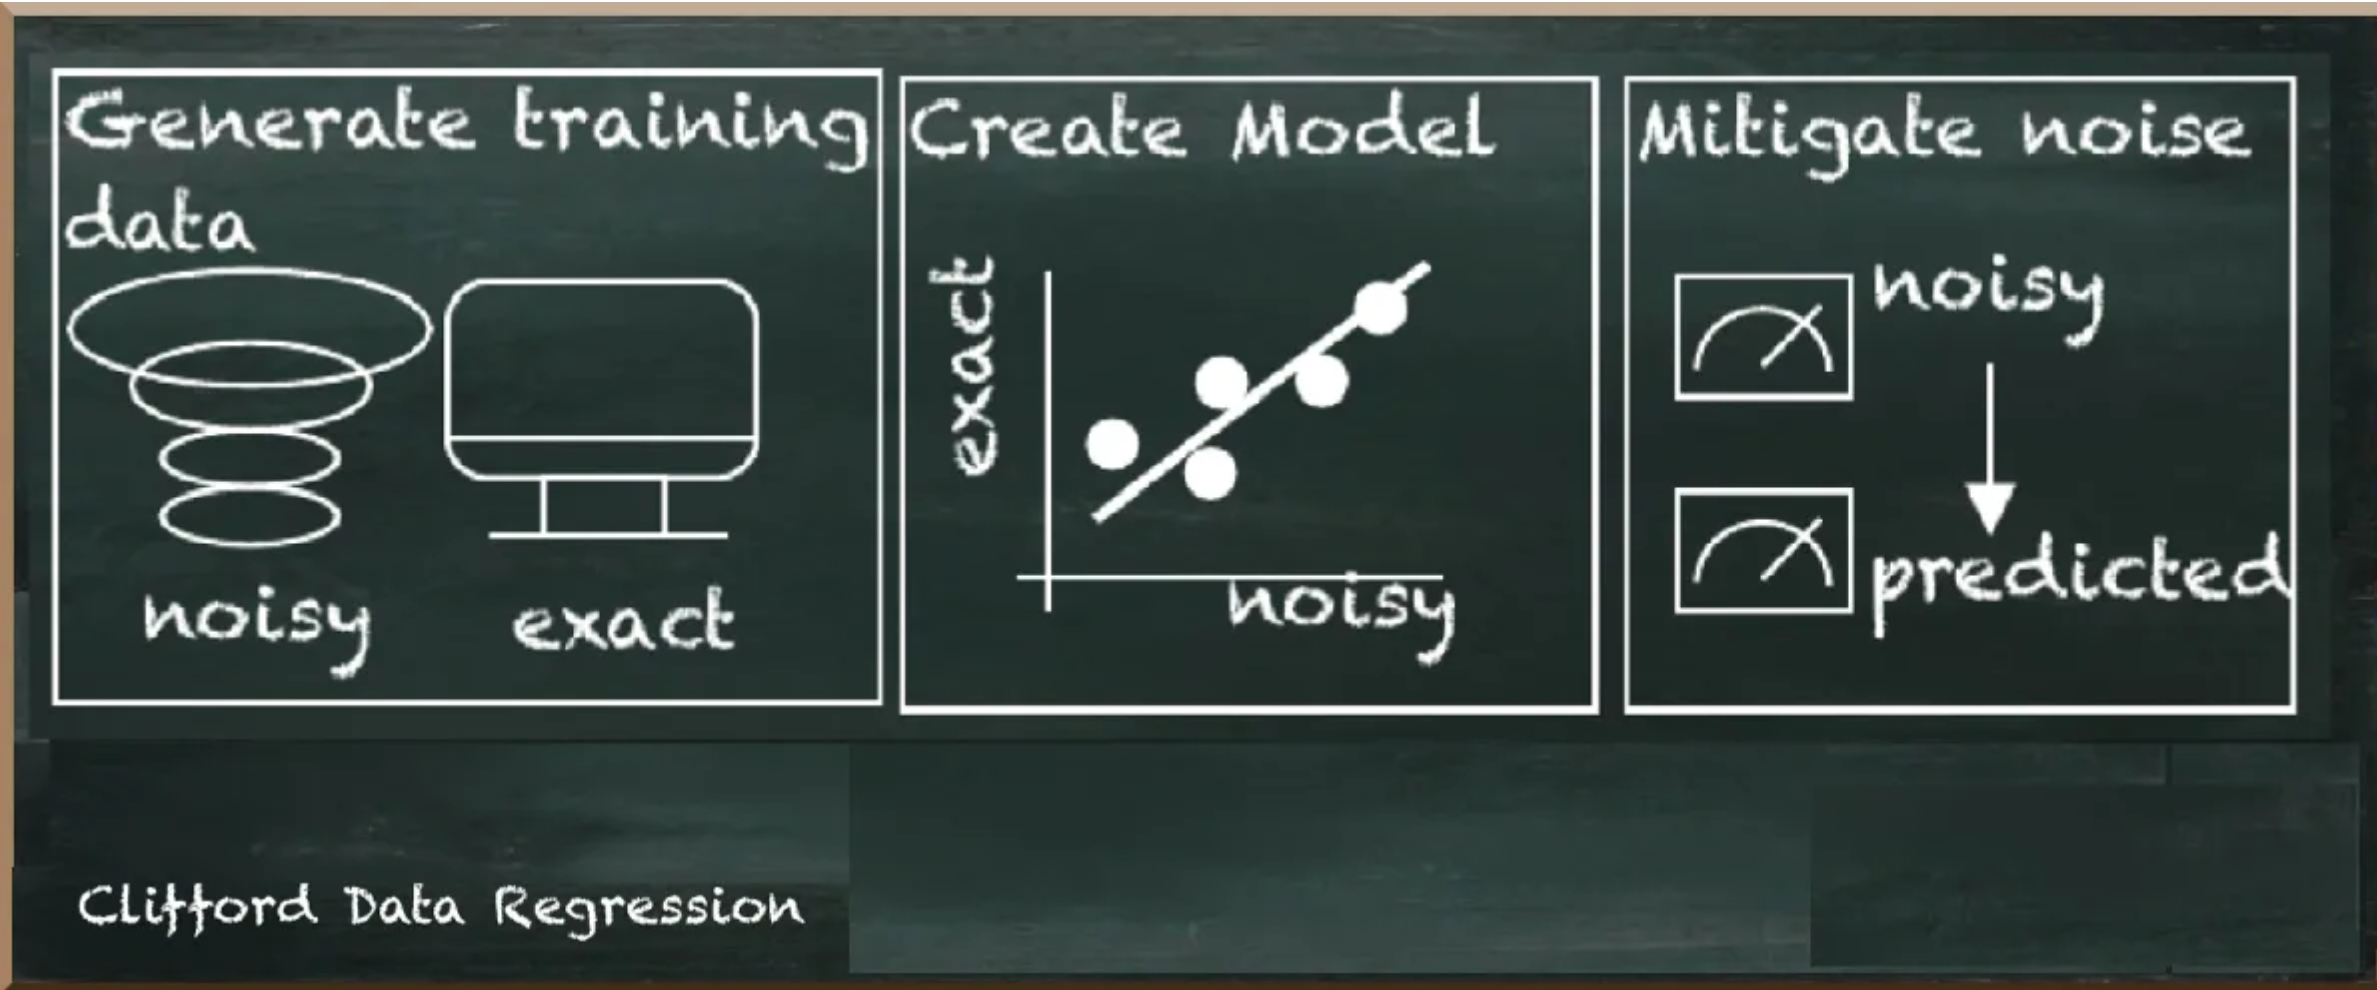
\includegraphics[width=0.7\linewidth]{Screenshot 2024-04-16 111314.png}
}
}
%%% Our strategy %%%%%%%%%%%%%%%%%%%%%%%%%%%%%%%%%%%%%%%%%%%%%%%%%%%%%%%%%%%%%%%%%%%%%
\headerbox{Our strategy}{name=OS,column=1,below=ML}{
In order to tap into QPU+HPC advantage over traditional density matrix formalism for calculating the discord, we need to pose the problem in a manner NISQ quantum computers are known to work. We aim to use the Quantum Discord tool both for quantifying correlation related spectroscopic effects and suggesting observation protocols for second quantum revolution relevant nC. We use classical shadow tomography with a selection of circuits with their quantum discord pre-calculated in a traditional computer. Although the calculations in traditional computers are heavy, they don't need to be repeated. Since quantum discord space is vast, we use ML methods to weight the impact of a particular circuit, and mitigate errors at the same time. The advantage of this approach is that the accuracy can be systematically improved as better quantum hardware and traditional alghoritms become available.   
    \center{
    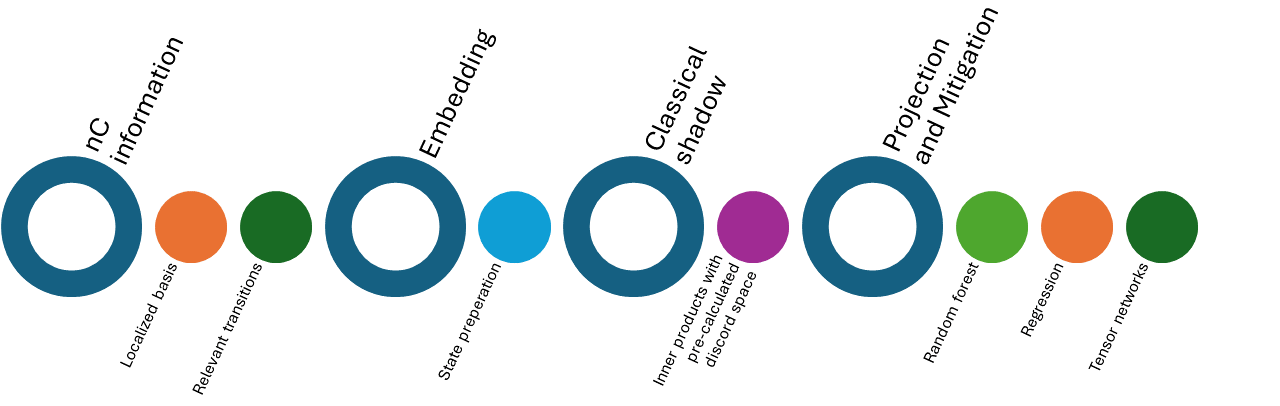
\includegraphics[width=1\linewidth]{strategy-QD.png}}
}
%%% Acknowledgeents %%%%%%%%%%%%%%%%%%%%%%%%%%%%%%%%%%%%%%%%%%%%%%%%%%%%%%%%%%%%%%%%%%%%%
\headerbox{Acknowledgements}{name=ack,column=1,below=OS,above=bottom}{
\small{The numerical calculations reported in this paper were partially performed at TUBITAK ULAKBIM, and in VEGA HPC through EuroHPC benchmark access.}  
}
\end{poster}
\end{document}
